\chapter[Maps]{Maps}
% \section{Geographical maps}
\begin{figure}  
\subfigure[Southeast Asia with West Papua\label{Figure_0.1}]{ 
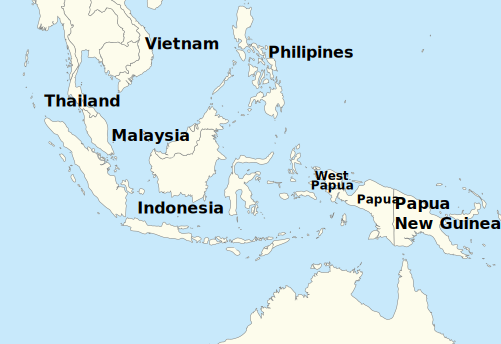
\includegraphics[height=4.7cm]{./figures/Indonesia}
}
\hfill
\subfigure[West Papua with its provinces Papua and Papua Barat\label{Figure_0.2}]{
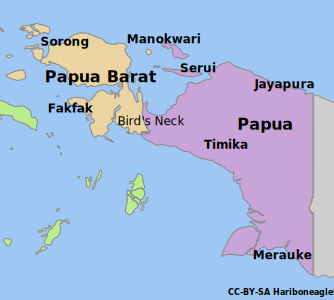
\includegraphics[height=4.7cm]{./figures/papua}
} 

\subfigure[\ili{Sarmi} regency with some of its towns and villages\label{Figure_0.3}]{ 
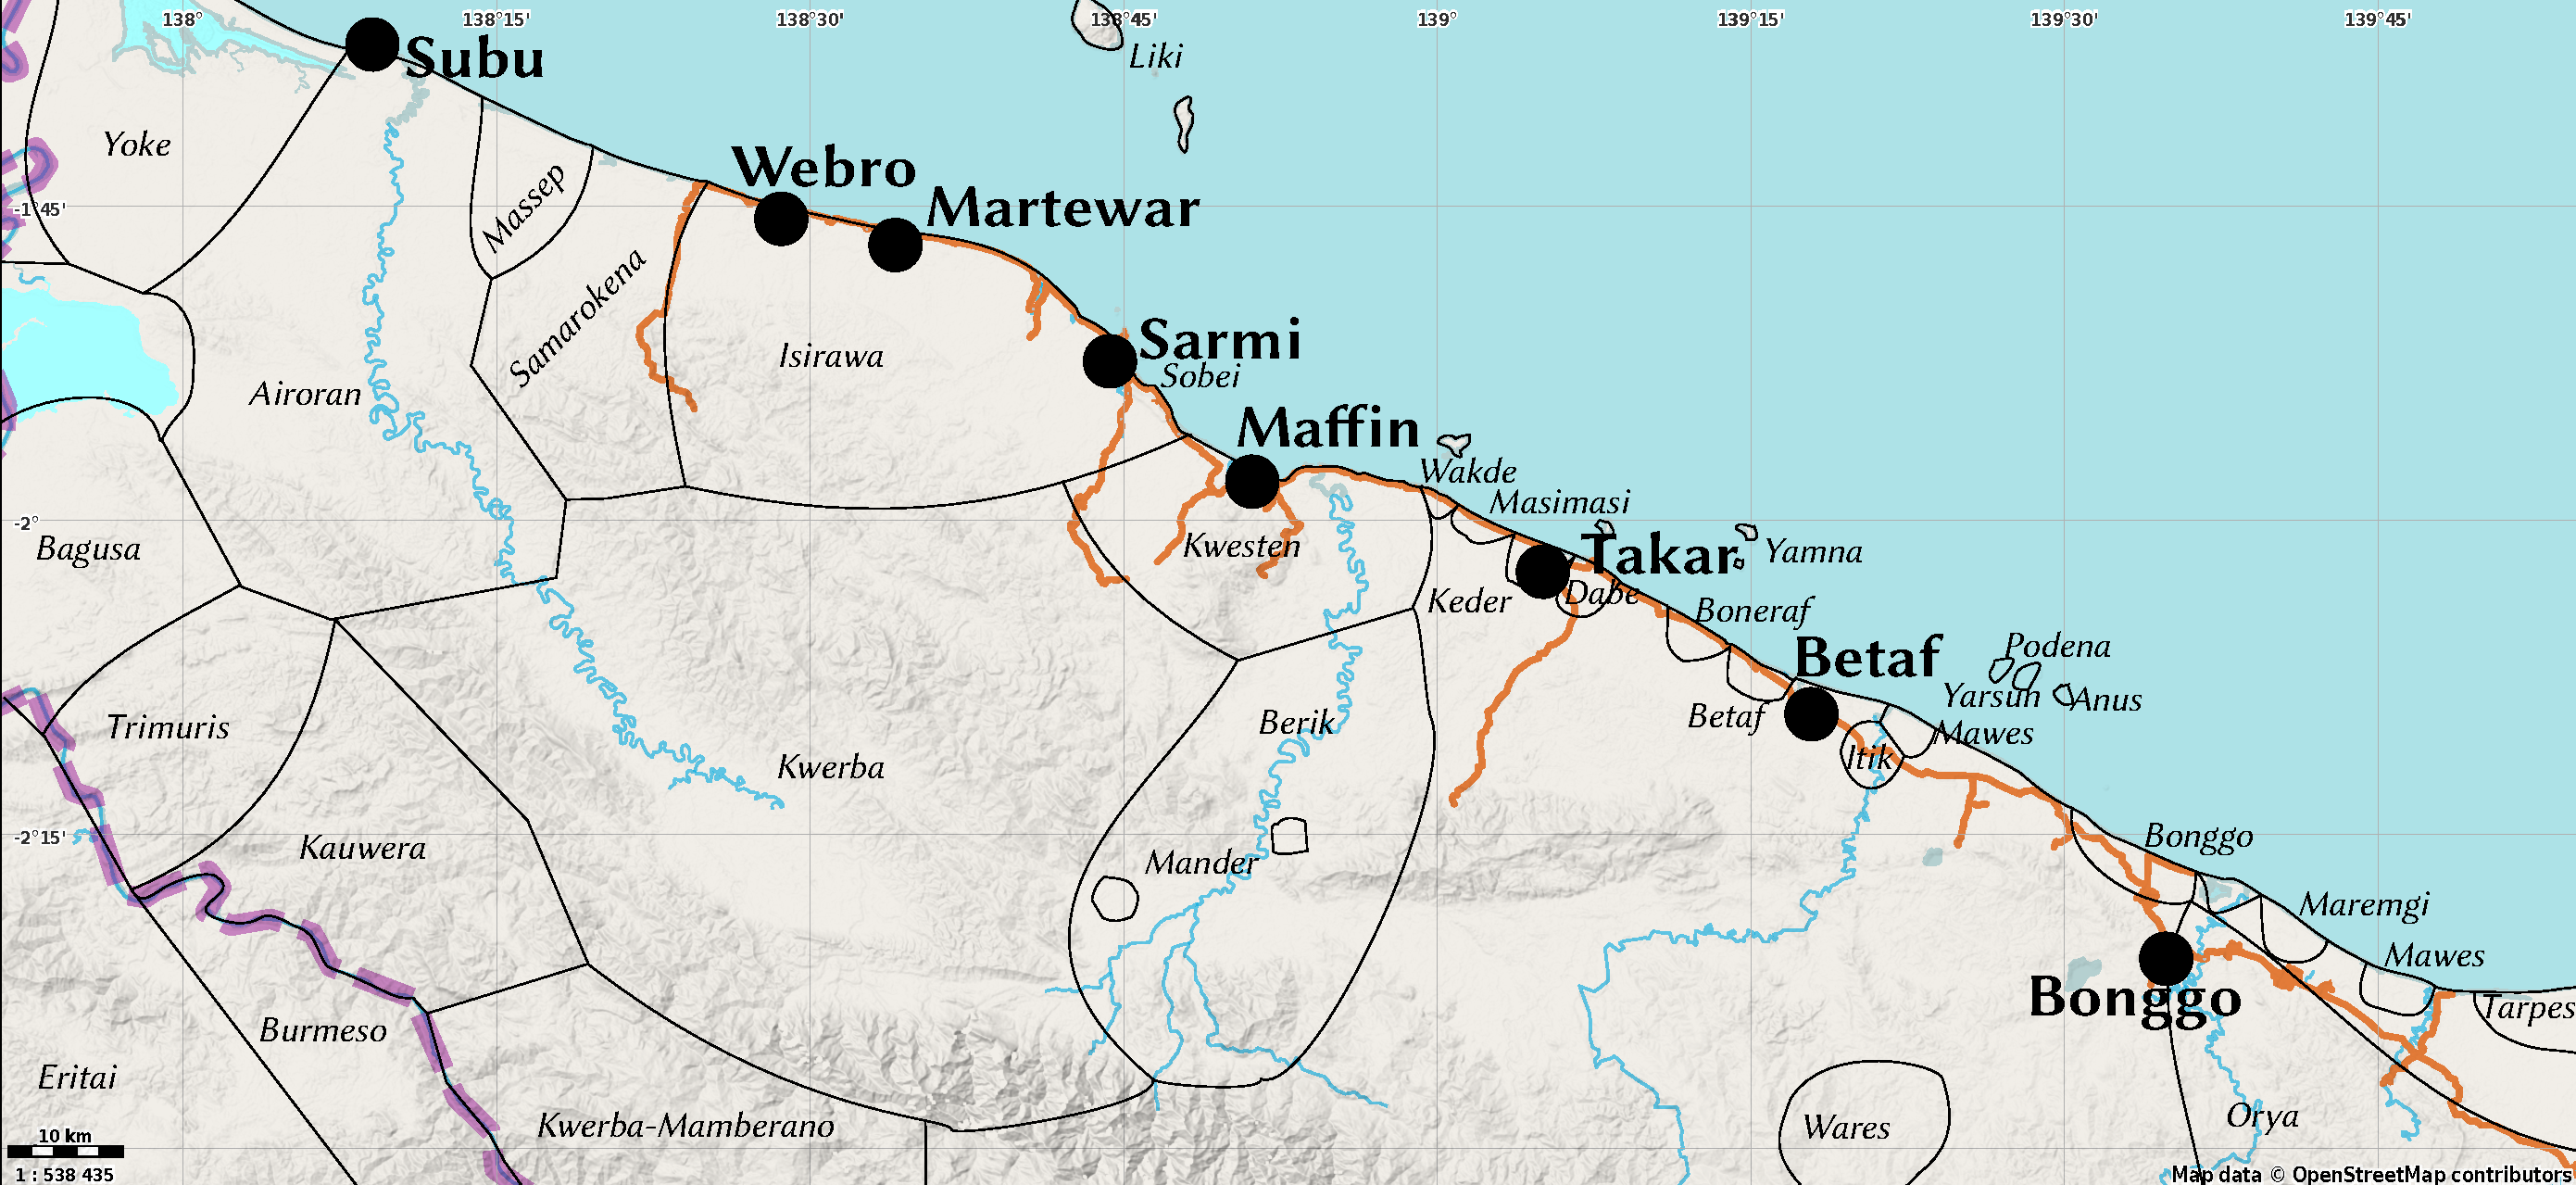
\includegraphics[width=.98\textwidth]{./figures/northcoast.pdf}
}

\caption{The location of the Sarmi regency within Southeast Asia and West Papua}
\end{figure}

% \section{Language map}
% 
% In \figref{Figure_0.4}, the \ili{Fedan} language is listed as \ili{Podena}, \ili{Dineor} as \ili{Maremgi}, \ili{Keijar} as \ili{Keder}, \ili{Mo} as \ili{Wakde}, and \ili{Sunum} as \ili{Yamna} (see §\ref{Para_1.4}).
% 
% \begin{figure}
% \centering
% 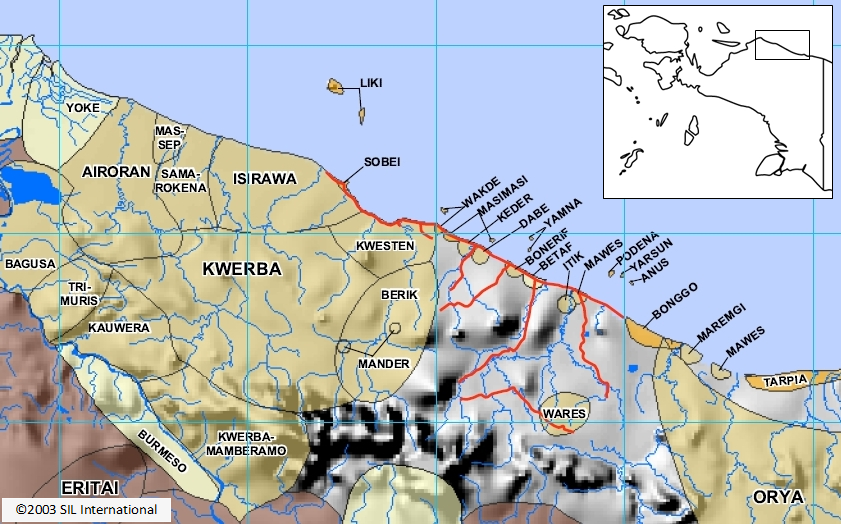
\includegraphics[scale=0.6, angle=90]{./figures/Figure_0_4}
% \caption{Austronesian and Papuan languages in the larger Sarmi region}\label{Figure_0.4}
% \end{figure}
